\section{Whole body motion for screwing}

The goal of this third behavior was to check if the humanoid robot HRP-2  is able to make the basic motion necessary to perform screwing action on the engine pylon. 
Note that an extender of 10 cm is suppose to be at the extremity of the electric screwdriver.

\begin{figure}
  \begin{center}
    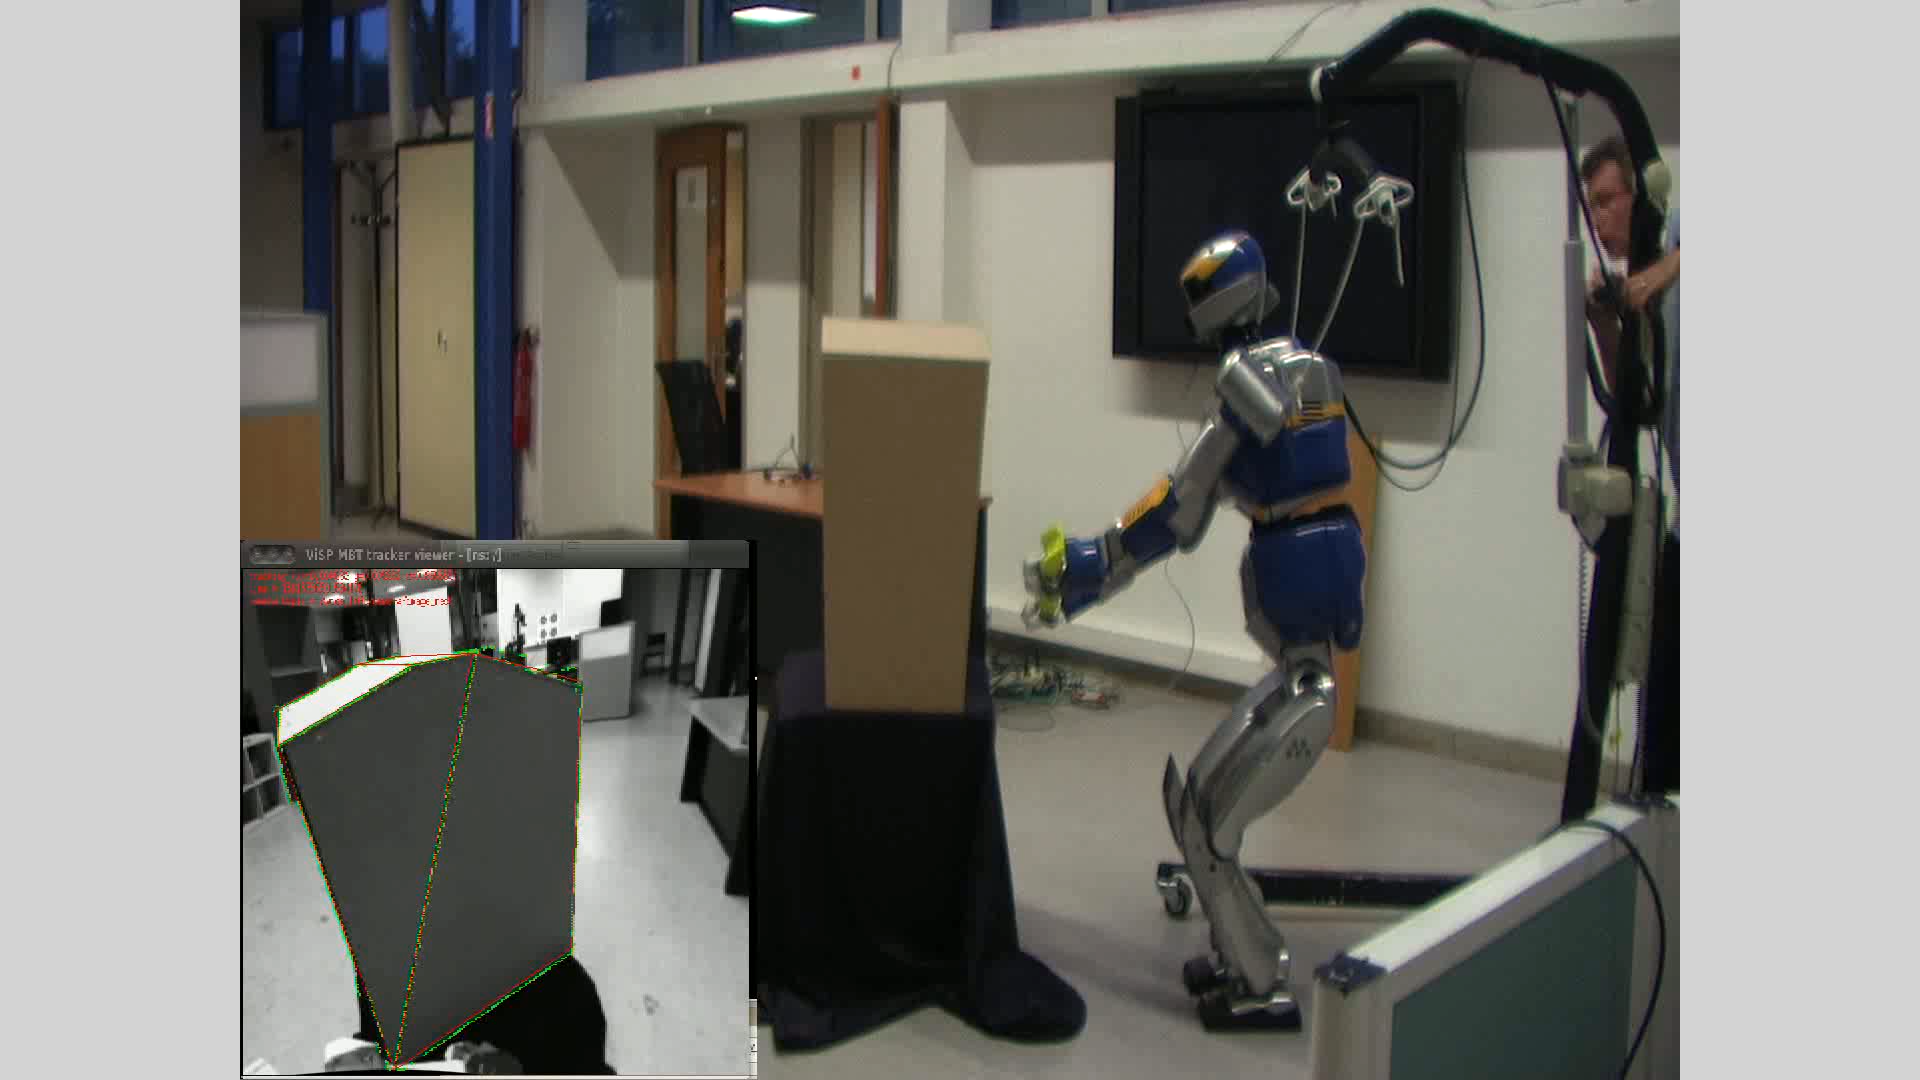
\includegraphics[clip=true, keepaspectratio, height=0.28\linewidth, trim={6.5cm 0cm 6.5cm 0cm}]{figures/engine_pylon_mockup.png}\hfill
    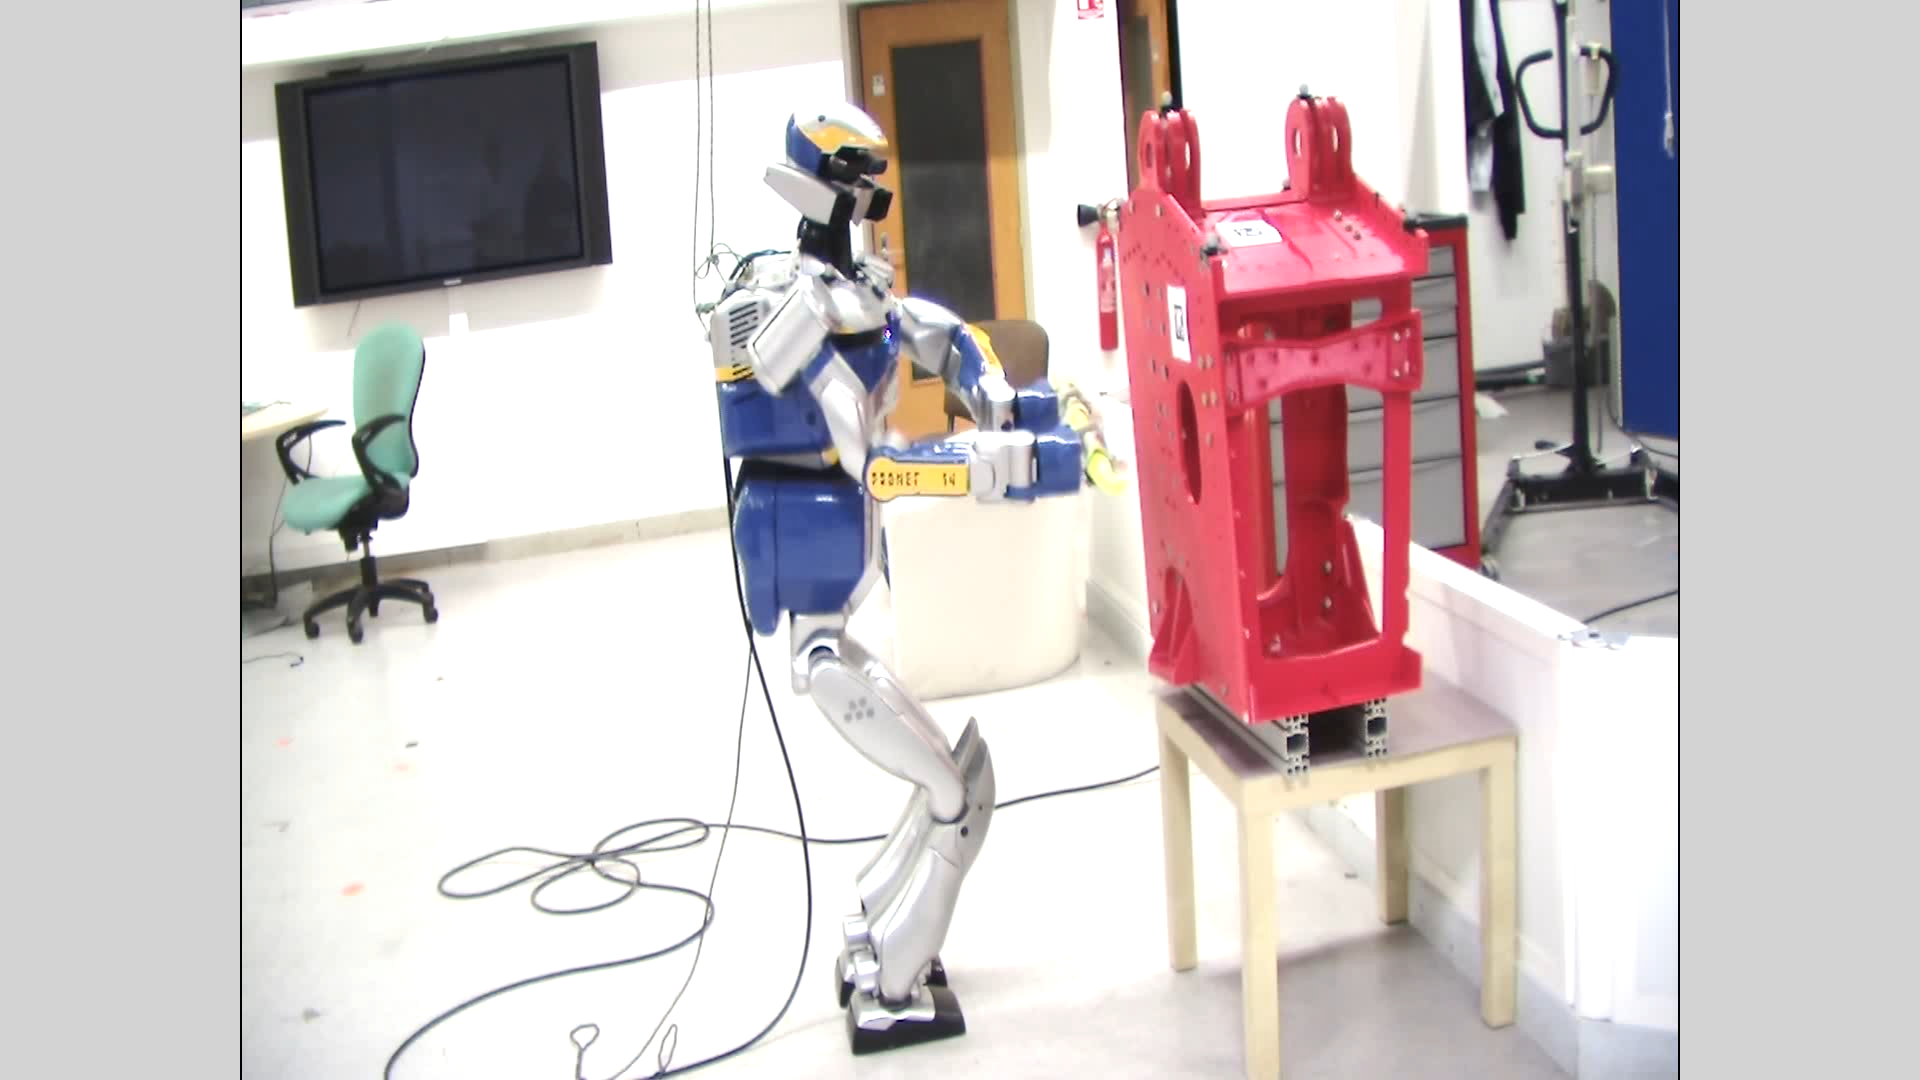
\includegraphics[clip=true, keepaspectratio, height=0.28\linewidth, trim={6.5cm 0cm 6.5cm 0cm}]{figures/whole_body_motion_engine_pylon.png}        
    % trim={<left> <lower> <right> <upper>}
  \end{center}
  \caption{HRP-2 doing a whole body screwing motion holding a 3D printed industrial screwdriver. On the left side one can see the visual servoing done on a mockup of the engine pylon. On the right side the robot is controlled via motion capture data as the visual servoing did not work on the 3D printed engine pylon.}
  \label{fig:whole:body:motion:screwing}
\end{figure}

The behavior realized was based on the stack of tasks \cite{mansard:icar:09} a framework which is combining different control laws together 
and takes advantage of humanoid robots redundancy. Its software implementation has been used since 2006 to implement various demonstrators. 
The goal of the mathematical formulation is to enforce properties which make the control safer by checking strictly some limits.
The efficiency is preserved and online changes of the control are till possible \cite{escande-ijrr-14}. 

In the frame of the PoC, the main point was to test the work space of the HRP-2 humanoid with a 3D print of an AIRBUS screwdriver.
The robot was able to reach most of the positions in the frontal plane of the engine pylon. 
On the wood mockup we have been able to realize a behavior where the robot is visually tracking the point by a whole body motion without moving the feet.
However the vision process did not work properly on the 3D-print, so we decided to switch to the Motion Capture.
This is demonstrated in the Fig.~\ref{fig:whole:body:motion:screwing}. 
It has to be noticed that the transition between the points is not formally proved or checked. 
It worked because the robot is highly redundant and we did not push the robot to the limit.
In order to reach the screws, we would need the plan the whole body trajectories offline.
During the process we have tested acceleration joint control to improve the behavior of the system.

The behavior was very much improved but we found one problem when using posture tasks. 
For this reason we came back to the usual kinematic control.
In addition we have tested very high gain showing that the robot is able to go up to $1.6 s$ between the transitions. 
The momentum involved by this fast motion cannot be recovered by the current robot stabilizer and still has to be taken into account at a higher level.
For this reason, we kept a rather low gain for the robot and 
we are currently in the process of improving it.
Finally we noted that when the robot is lowering down it is close to self-collision. 
This can be fixed by using self-collision avoidance, however it calls for a deep interaction between planning and control.
This is especially true when using vision. A slight drift in rotation may prevent the convergence
of the controller to a screwing point.

